\documentclass[a4paper,ngerman]{scrartcl}

\usepackage[utf8]{inputenc}

\usepackage[ngerman]{babel}

\usepackage{amsmath,amsthm,amssymb,stmaryrd,color,graphicx}
\usepackage{bussproofs}
\usepackage{array}
\usepackage{comment}

\usepackage[protrusion=true,expansion=true]{microtype}

\usepackage{lmodern}
\usepackage{tabto}

%\usepackage[natbib=true,style=numeric]{biblatex}
%\usepackage[babel]{csquotes}
%\bibliography{literatur}

\usepackage[all]{xy}

\usepackage{hyperref}

\setlength\parskip{\medskipamount}
\setlength\parindent{0pt}

\theoremstyle{definition}
\newtheorem{defn}{Definition}[section]
\newtheorem{bsp}[defn]{Beispiel}

\theoremstyle{plain}

\newtheorem{prop}[defn]{Proposition}
\newtheorem{motto}[defn]{Motto}
\newtheorem{ueberlegung}[defn]{Überlegung}
\newtheorem{lemma}[defn]{Lemma}
\newtheorem{kor}[defn]{Korollar}
\newtheorem{hilfsaussage}[defn]{Hilfsaussage}
\newtheorem{satz}[defn]{Satz}

\theoremstyle{remark}
\newtheorem{bem}[defn]{Bemerkung}
\newtheorem{aufg}[defn]{Aufgabe}

\clubpenalty=10000
\widowpenalty=10000
\displaywidowpenalty=10000

\newcommand{\xra}[1]{\xrightarrow{#1}}
\newcommand{\lra}{\longrightarrow}
\newcommand{\lhra}{\ensuremath{\lhook\joinrel\relbar\joinrel\rightarrow}}
\newcommand{\thlra}{\relbar\joinrel\twoheadrightarrow}

\newcommand{\ZZ}{\mathbb{Z}}
\newcommand{\QQ}{\mathbb{Q}}
\newcommand{\RR}{\mathbb{R}}
\newcommand{\NN}{\mathbb{N}}
\newcommand{\PP}{\mathbb{P}}
\newcommand{\I}{\mathcal{I}}
\newcommand{\C}{\mathcal{C}}
\newcommand{\D}{\mathcal{D}}
\newcommand{\E}{\mathcal{E}}
\renewcommand{\I}{\mathcal{I}}
\renewcommand{\P}{\mathcal{P}}
\renewcommand{\O}{\mathcal{O}}
\newcommand{\Hom}{\mathrm{Hom}}
\newcommand{\ev}{\mathrm{ev}}
\newcommand{\id}{\mathrm{id}}
\newcommand{\Id}{\mathrm{Id}}
\newcommand{\freist}{\underline{\ \ }}
\DeclareMathOperator{\colim}{colim}
\DeclareMathOperator{\Ob}{Ob}
\DeclareMathOperator{\ggT}{ggT}
\newcommand{\op}{\mathrm{op}}
\newcommand{\Set}{\mathrm{Set}}
\newcommand{\Grp}{\mathrm{Grp}}
\newcommand{\Vect}[1]{{#1\text{-}\mathrm{Vect}}}
\newcommand{\AbGrp}{\mathrm{AbGrp}}
\newcommand{\Ring}{\mathrm{Ring}}
\newcommand{\Cat}{\mathrm{Cat}}
\newcommand{\Funct}{\mathrm{Funct}}
\newcommand{\Eins}{\mathbf{1}}
\newcommand{\Man}{\mathrm{Man}}
\newcommand{\Top}{\mathrm{Top}}
\newcommand{\seq}[1]{\mathrel{\vdash\!\!\!_{#1}}}

\newcommand{\XXX}[1]{\textcolor{red}{#1}}

\renewcommand*\theenumi{\alph{enumi}}
\renewcommand{\labelenumi}{\theenumi)}

\newcommand\subsubsubsection[1]{\subsubsection*{#1}}
\definecolor{grey}{rgb}{0.7,0.7,0.7}

\setcounter{tocdepth}{2}

\newenvironment{indentblock}{%
  \list{}{\leftmargin\leftmargin}%
  \item\relax
}{%
  \endlist
}


%Zusätzliche Befehle (Lukas)
\newcommand{\Stirling}[2]{\left\lbrace\begin{matrix}#1 \\ #2\end{matrix}\right\rbrace}
\newcommand{\SZwei}{\mathrm{S}\!\!2}
\newcommand{\dd}{\mathrm{d}}


%\newarrow{Equals}=====

%\usepackage{geometry}
%\geometry{tmargin=2cm,bmargin=4cm,lmargin=3cm,rmargin=3cm}

\begin{document}

\vspace*{2em}%
\begin{center}%
  \vskip 1em
  {\LARGE Pizzaseminar zu erzeugenden Funktionen}
  \vskip 1.5em%
  {\large
   \lineskip .5em%
    \begin{tabular}[t]{c}%
      \today
    \end{tabular}\par}%
    \vskip 1em%
\end{center}\par
\par\vskip 1.5em

\begin{center}\emph{in Entstehung befindlich} \\ \ \\
\end{center}


\subsection{Multivariate erzeugende Funktionen}

\subsubsubsection{Allgemeines Verfahren:}
\begin{description}
	\item[1. Schritt:] Geeignete Rekursion finden
	\item[2. Schritt:] Erzeugende Funktion erstellen
	\item[3. Schritt:] Rekursion für Funktion
	\item[4. Schritt:] Formel auflösen

\end{description}

Geeignete Funktionen für den 2. Schritt (für den Fall zweier Variablen):
\[\psi(x,y) = \sum_{n,k \geq 0} a_{n,k} x^n y^k\]
\[\phi(x,y) = \sum_{n,k \geq 0} a_{n,k} \frac{x^n}{n!} \frac{y^k}{k!}\]
\[\theta(x,y) = \sum_{n,k \geq 0} a_{n,k} \frac{x^n}{n!} y^k\]

\begin{bsp}
Der Binomialkoeffizient
\[f(n,k) := \left(\begin{matrix} n \\ k\end{matrix}\right) := \frac{n!}{(n-k)!k!}\]
entspricht der Anzahl der $k$-elementigen Teilmengen der $n$-elementigen Menge $\{1, \dots, n\}$.
\begin{description}
	\item[1. Schritt]
		Eine $k$-elementige Teilmenge von $\{1, \dots, n\}$ ist entweder auch eine $k$-elementige Teilmenge von $\{1, \dots, n-1\}$ (wenn $n$ nicht in der Teilmenge enthalten ist) oder eine $(k-1)$-elementige Teilmenge von $\{1, \dots, n-1\}$ vereinigt mit $\{n\}$. Somit erhält man die Rekursion:
		\begin{align*}
			f(n,k) &:= f(n-1,k) + f(n-1,k-1), 	&n,k \geq 1 \\
			f(0,k) &:= 0, 						&k \geq 1   \\
			f(n,0) &:= 1						&n \geq 0
		\end{align*}
	\item[2. Schritt]
		\begin{align*}\psi(x,y) := \sum_{n,k \geq 0} f(n,k) x^n y^k \end{align*}
	\item[3. Schritt]	
		\begin{align*}
			\psi(x,y) 	&= \sum_{n,k \geq 0} f(n,k) x^n y^k = \\
						&= \sum_{k \geq 1} f(0,k) x^0 y^k + \sum_{n \geq 1} f(n,0) x^n y^0 + \sum_{n,k \geq 1} f(n,k) x^n y^k = \\
						&= 0 + \frac{1}{1-x} + \sum_{n,k \geq 1} f(n-1,k) x^n y^k + \sum_{n,k \geq 1} f(n-1,k-1) x^n y^k = \\
						&= \frac{1}{1-x} + x\sum_{n,k \geq 0} f(n,k) x^n y^k - \sum_{n \geq 0} f(n,0) x^n y^0 + xy\sum_{n,k \geq 0} f(n,k) x^n y^k = \\
						&= \frac{1}{1-x} + x\psi(x,y) - \frac{x}{1-x} +xy\psi(x,y) = x\psi(x,y) + xy\psi(x,y) 
		\end{align*}
	\item[4. Schritt]
		Umformen von
		\[\psi(x,y) = x\psi(x,y) + xy\psi(x,y)\]
		ergibt
		\[\psi(x,y)(1-x-xy) = 1\]
		und damit die erzeugende Funktion
		\[\psi(x,y) = \frac{1}{1-x-xy}\]
\end{description}

Was passiert nun, wenn eine Variable fest ist?

\begin{description}
	\item[1. Fall: n fest]
	\begin{align*}
		B_n(y) 	&= \sum_{k \geq 0} f(n,k)y \\
	x^k f(n,k) 	&= x^k f(n-1,k) + x^k f(n-1,k-1) \\
		B_n(x) 	&= \sum_{k \geq 0} x^k f(n,k) = \sum_{k \geq 0} x^k f(n-1,k) + \sum_{k \geq 0} f(n-1,k -1) x^k = \\	
				&= B_{n-1}(x) + x B_{n-1}(x) \\
		\Rightarrow B_n(x) &= (1+x)B_{n-1}(x) \\
		\Rightarrow B_n(x) &= (1+x)^n \\
		\Rightarrow f(n,k) &= [x^k] (1+x)^n = \left.\frac{n(n-1)\dots(n-k+1)(1+x)^{n-k}}{k!}\right|_{x=0} = \\
				&= \frac{n(n-1) \dots (n-k+1)}{k!} = \frac{n!}{k!(n-k)!}
	\end{align*}

	\item[2. Fall: k fest]
	\[F_k(x) = \sum_{n \geq 0} \left(\begin{matrix}x \\ k\end{matrix}\right) x^n = [y^k]\psi(x,y) = [y^k] \frac{1}{1-x-xy} = \frac{1}{1-x}[y^k]\frac{1-x}{1-x-xy} = \dots = \frac{x^k}{(1-x)^{k+1}}\]
	\[\theta(x,y) = \sum_{n,k \geq 0}f(n,k)\frac{x^n}{n!}y^k = \sum_{n,k \geq 0} \left(\begin{matrix}x \\ k\end{matrix}\right) \frac{x^n}{n!}y^k = \XXX{???} \]

\end{description}
\end{bsp}


\begin{bsp}[Delannoy-Zahlen]
Die Delannoy-Zahl $\omega_{n,k}$ gibt die Anzahl der Möglichkeiten an in einem kartesischen Koordinatensystem vom Punkt $(0,0)$ zum Punkt $(n,k)$ zu gelangen. Dabei sind nur Schritte nach rechts, rechtsoben und oben erlaubt:

\begin{figure}[h]\begin{center}
	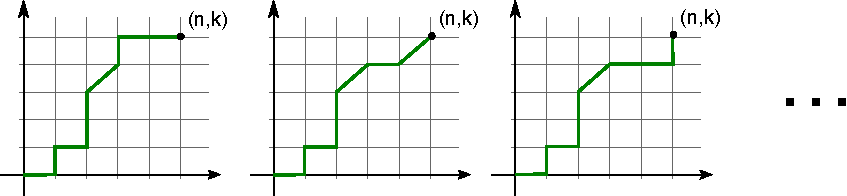
\includegraphics[width=0.8\textwidth]{Delannoy-Zahlen.pdf}
	\caption{\footnotesize Verschiedene Wege vom Ursprung zum Punkt $(n,k)$}
\end{center}\end{figure}
\begin{description}
	\item[1. Schritt]	
		Um eine Rekursionsformel für $\omega_{n,k}$ zu erhalten, betrachte alle Wege, die vom Ursprung nach $(n-1,k)$, $(n-1,k-1)$ oder $(n,k-1)$ führen. Von diesen drei Punkten aus wird $(n,k)$ in genau einem Schritt erreicht. Also entspricht die Summe dieser Wege der Zahl aller Wege von $(0,0)$ nach $(n,k)$:
		\begin{align*}
		\omega_{n,k} &:= \omega_{n-1,k} + \omega_{n-1,k-1} + \omega_{n,k-1}, 	&n,k \geq 1 \\
		\omega_{0,k} &:= \omega_{n,0} = \omega_{0,0} = 1						&n,k \geq 0
		\end{align*}
	\item[2./3. Schritt]
		\begin{align*}
			\psi(x,y) 	&= \sum_{n,k \geq 0} \omega_{n,k} x^n y^k \\
						&= \omega_{0,0} + \sum_{n\geq 1} \omega_{n,0} x^n + \sum_{k\geq 1} \omega_{0,k}y^k \\
						&\qquad{}+ \sum_{n,k \geq 1} \omega_{n-1,k} x^n y^k + \sum_{n,k \geq 1} \omega_{n-1,k-1} x^n y^k + \sum_{n,k \geq 1} \omega_{n,k-1} x^n y^k \\
						&= 1 + \frac{x}{1-x} + \frac{y}{1-y}  \\
						&\qquad {}+ x\sum_{n,k \geq 0} \omega_{n,k} x^n y^k - x \sum_{n \geq 0} \omega_{n,0} x^n + xy \sum_{n,k \geq 0} \omega_{n,k} x^n y^k + y \sum_{n,k \geq 0} \omega_{n,k} x^n y^k - y \sum_{k \geq 0} \omega_{0,k} y^k \\
						&= 1 + \frac{x}{1-x} + \frac{y}{1-y} + x\psi(x,y) - \frac{x}{1-x} + xy\psi(x,y) + y\psi(x,y) - \frac{y}{1-y} \\
						&= 1 + x\psi(x,y) - xy\psi(x,y) + y\psi(x,y)
		\end{align*}
	\item[4. Schritt]		
		\[\Rightarrow \psi(x,y) = \frac{1}{1-x-y-xy}\]
\end{description}
\end{bsp}


\begin{bsp}[Stirlingzahlen 2. Art]
Die Stirlingzahlen 2. Art sind wie folgt definiert:
\[S(n,k) := \Stirling{n}{k} := \text{ Anzahl der Partitionen einer }n\text{-elementigen Menge in }k\text{ Teile (nicht-leere Mengen)}\]
Beispielsweise ist 
\[\{1,2\}, ~ \{13\}, ~ \{3,5,8,12\}, ~ \{4,6\}, ~ \{7,9,10,11\}\]
eine mögliche Partition von $\{1, \dots, 13\}$ in 5 Teile.

\begin{description}
	\item[1. Schritt]
		Eine $k$-Partition von $\{1, \dots, n\}$ erhält man entweder aus einer $k$-Partition von $\{1, \dots, n-1\}$ durch Hinzufügen von $n$ in eine der $k$ Partitionen oder aus einer $(k-1)$-Partition von $\{1, \dots, n-1\}$ durch Hinzufügen von $\{13\}$ als eigener Menge:
		\begin{align*}
		\Stirling{n}{k} &:= k \Stirling{n-1}{k} + \Stirling{n-1}{k-1},	&n, k \geq 1 \\
		\Stirling{0}{k} &:= 0, ~ \Stirling{n}{0} := 0, 				&n,k \geq 1  \\
		\Stirling{0}{0} &:= 1
		\end{align*}


	\item[2./3. Schritt]
		\begin{align*}
		\SZwei(x,y) &= \sum_{k,n \geq 0} \Stirling{n}{k} \frac{x^n}{n!} y^k = 1 + \sum_{k,n \geq 1} \Stirling{n}{k} \frac{x^n}{n!} y^k = \\
				&= 1 + \sum_{k,n \geq 1} k\Stirling{n-1}{k} \frac{x^n}{n!} y^k + \sum_{k,n \geq 1} \Stirling{n-1}{k-1} \frac{x^n}{n!} y^k = \\
				&= 1 + \sum_{n,k \geq 0}\Stirling{n}{k} \frac{x^{n+1}}{(n+1)!} y^k + y \sum_{n,k \geq 0} \Stirling{n}{k}\frac{x^{n+1}}{(n+1)!} y^k = \\
				&= y\frac{\dd}{\dd y} \int_0^x\SZwei(x,y)\dd x + y\int_0^x\SZwei(x,y)\dd x
		\end{align*}


	\item[4. Schritt]
		Wende auf beide Seiten $\frac{\dd}{\dd x}$ an
		\[\frac{\dd}{\dd x} \SZwei(x,y) = y\left(\frac{\dd}{\dd y}\SZwei(x,y) + \SZwei(x,y)\right)\]
		substituiere $\SZwei(x,y) = e^{f(x,y)}$ und teile durch $e^{f(x,y)}$:
		\[\frac{\dd}{\dd x} f(x,y) = y\left(\frac{\dd}{\dd y}f(x,y) + 1\right)\]
		Substituiere $f(x,y) = g(x,y)-y$:
		\[\frac{\dd}{\dd x} g(x,y) = y\frac{\dd}{\dd y}g(x,y)\]
		Substituiere $g(x,y) = u(x)v(y)$:
		\[u'(x)v(y) = y u(x)v'(y)\]
		\[\Rightarrow \frac{u'(x)}{u(x)} = y\frac{v'(y)}{v(y)}\]
		\[\Rightarrow u(x) = ce^{x},~ v(y) = y\]
		Daraus ergibt sich $g(x,y) = c y e^{x}$, also $f(x,y) = c y e^{x} - y$ und somit:
		\[\SZwei(x,y) = e^{f(x,y)} + K = e^{cye^{x}-y} - y + K\]
		Aus den Anfangsbedingung folgt $K = 0$ und $c = 0$, also:
		\[\SZwei(x,y) = e^{y(e^{x} -1)}\]
		
\end{description}

\end{bsp}

Damit ergibt sich auch die Erzeugende für die Bell-Zahlen: 
\[\SZwei(x,1) = e^{(e^{x} -1)}\]


%Sage:
%R.<x> = PowerSeriesRing(QQ)
%i= 0
% For c in exp(exp(x)-1).coefficiens():
%	print c*factorial(i)
%	i=i+1


%\nocite{*}
%\printbibliography

\end{document}
